%!TEX program = pdflatex
% Full chain: pdflatex -> bibtex -> pdflatex -> pdflatex
\documentclass[11pt,en]{elegantpaper}


\definecolor{codegreen}{rgb}{0,0.6,0}
\definecolor{codegray}{rgb}{0.5,0.5,0.5}
\definecolor{codepurple}{rgb}{0.58,0,0.82}
\definecolor{backcolour}{rgb}{0.95,0.95,0.92}

\lstdefinestyle{mystyle}{
	backgroundcolor=\color{backcolour},   
	commentstyle=\color{codegreen},
	keywordstyle=\color{magenta},
	numberstyle=\tiny\color{codegray},
	stringstyle=\color{codepurple},
	basicstyle=\ttfamily\footnotesize,
	breakatwhitespace=false,         
	breaklines=true,                 
	captionpos=b,                    
	keepspaces=true,                 
	numbers=left,                    
	numbersep=5pt,                  
	showspaces=false,                
	showstringspaces=false,
	showtabs=false,                  
	tabsize=2
}

\lstset{style=mystyle}


\title{Investigación reproducible \\ Buenas prácticas para el manejo de datos y códigos\footnote{Traducción al español a cargo de: Sebastián Hernández y Rony Rodríguez-Ramírez.}}
\author{Harrison Diamond Pollock \and Erica Chuang \and Stephanie Wykstra}
\date{\today}


\begin{document}
%----------------------------------------------------------------------------------------
\maketitle
\tableofcontents
%----------------------------------------------------------------------------------------
\newpage 
\section{Introducción}
\label{sec:intro}
%----------------------------------------------------------------------------------------

Las revistas, los financiadores de investigación y los grupos de investigación como Innovations for Poverty Action reconocen cada vez más el valor de la transparencia en la investigación. La transparencia de la investigación incluye el registro previo de estudios y el intercambio de materiales como datos y códigos para permitir que otros vuelvan a analizar los resultados informados.

La gestión adecuada de datos y códigos durante un proyecto es esencial para la transparencia después de la finalización de un proyecto. También son importantes para uso interno, ya que los proyectos a menudo se ejecutan durante varios años, con varios miembros del personal trabajando en ellos de forma secuencial.

Esta guía describe las mejores prácticas en el manejor de datos y códigos. El alcance de la guía es cubrir los principios de organización y documentación de materiales en todos los pasos del ciclo de vida de un proyecto con el objetivo de hacer que la investigación sea reproducible. La guía no cubre las mejores prácticas para diseñar encuestas, limpiar datos o realizar análisis de datos. En cada sección, explicamos el "qué", el "por qué" y el "cómo" de cada práctica recomendada.

Para comentarios/preguntas, comuníquese con \href{mailto:researchsupport@poverty-action.org}{researchsupport@poverty-action.org}.

%----------------------------------------------------------------------------------------
\newpage 
\section{Estructura de carpetas y archivos}
\label{sec:estructura}
%----------------------------------------------------------------------------------------
\noindent
\textbf{¿Qué?}

La estructura de carpetas describe la organización de las carpetas que contienen todos los archivos del proyecto. Por lo general, las carpetas se designan para ciertos tipos de archivos (e.g., do-files, archivos de datos, tablas, etc.), así como puntos en el tiempo (e.g., línea de base, línea media, línea final).

\noindent
\textbf{¿Por qué?} 

Mantener una estructura de carpetas lógica significa que es mucho más fácil encontrar los archivos que está buscando. También facilita enormemente compartir un proyecto con otras personas, como los investigadores principales (PI, por sus siglas en inglés) y los nuevos asistentes de investigación (RA, por sus siglas en inglés) que trabajan en un proyecto. Tener un conjunto desorganizado de archivos significa que las transiciones de proyectos se vuelven mucho más difíciles

\noindent
\textbf{¿Cómo?}

\hyperref[fig:carpetas]{Aquí} un ejemplo de una estructura de carpetas describe una división lógica de archivos para un proyecto de investigación completo, y \hyperref[fig:code]{aquí} hay una estructura de carpetas recomendada para archivos de datos y códigos. 

Independientemente de la estructura de carpetas específica que usted decida, es fundamental \textbf{definirla de antemano} y limitar los archivos que necesita mantener (especialmente las base de datos) solo a aquellos que son estrictamente necesarios. Si desea mantener archivos extras/antiguos, es una buena práctica crear una carpeta "Archivo" donde se almacenan. \hyperref[sec:doorganizar]{Ver más abajo}.

¿Qué hay de heredar una estructura de carpetas existente? Si bien el caso ideal sería reorganizar los archivos y carpetas para que se ajusten a una estructura como la descrita anteriormente, es probable que sea un paso poco práctico y que requiera mucho tiempo. Antes de realizar cualquier cambio, un RA necesitaría un amplio conocimiento de la estructura actual y la relación entre los archivos. Crear un \textbf{mapa de carpetas} es una práctica recomendable en este caso. Este mapa (en Excel/Word) resumiría las carpetas clave en la estructura y qué archivos se encuentran dentro de ellas. Dicho documento formaría la base del \href{http://www.poverty-action.org/research-transparency/example-readme-files}{ReadME} del proyecto y resultará útil durante todo el ciclo de vida del proyecto.

\textbf{Nota:} Mantenga los nombres de archivos y carpetas simples y, siempre que sea posible, sin espacios.

%----------------------------------------------------------------------------------------
\newpage 
\section{Mejores prácticas para códigos}
\label{sec:practicas}
%----------------------------------------------------------------------------------------

%----------------------------------------------------------------------------------------
\subsection{Nombrar y etiquetar variables}
\label{sec:variables}
%----------------------------------------------------------------------------------------
\noindent
\textbf{¿Qué?}

Los nombres de las variables deben estar en un formato consistente. Las etiquetas deben aplicarse a todas las variables en un formato consistente. Las etiquetas de valor también son necesarias para algunas variables.

\noindent
\textbf{¿Por qué?} 

Sin nombres y etiquetas claros, sería muy difícil entender tus datos. Estas proporcionan información esencial sobre las variables, sin tener que volver a mirar cómo se construyeron. Incluir números de preguntas y\/o texto en las etiquetas de variables permite vincular la base de datos con el cuestionario original.

\noindent
\textbf{¿Cómo?} 

Las etiquetas de las variables deben adjuntarse a todas las variables una vez que se importen a Stata. Esto se puede hacer de varias maneras. Si está ejecutando una encuesta ODK / SurveyCTO, usando el comando odkmeta etiquetará sus variables con la etiqueta correspondiente que ha definido en el formulario ODK. De lo contrario, puede definir etiquetas manualmente en Stata. Además, no olvide \textbf{etiquetar las variables que cree después de la importación inicial}, como durante la limpieza y el análisis de datos.

Consulte este recurso sobre etiquetado variable para obtener más información sobre los convenios de \href{https://www.poverty-action.org/sites/default/files/Naming-and-Labeling-Data.pdf}{etiquetado} adecuados. En resumen, hay dos opciones principales para etiquetar en relación con el nombre de la variable. Si bien cualquiera de los dos puede usarse, asegúrese de elegir uno formatear y mantenerlo en todo momento.

\begin{itemize}
	\item Asigne una etiqueta descriptiva corta, mientras que el nombre de la variable hace referencia al número de pregunta del cuestionario.
	
	\item Asigne una etiqueta descriptiva corta que incluya el número de la pregunta, siendo el nombre de la variable descriptivo en sí.
\end{itemize}

\textbf{Nota:} Si una variable proviene directamente de un cuestionario, se debe establecer un vínculo claro entre el respectivo texto de pregunta y la variable. Incluir el texto de la pregunta en la etiqueta podría funcionar bien. Sin embargo, hay un límite de 80 caracteres en la longitud de la etiqueta. En tal caso, recomendamos incluir el texto de las preguntas como una \textbf{nota} variable.

Asignar nombres de variables adecuados también es importante. Como se describió anteriormente, los nombres de las variables pueden tomar varias formas. Si necesitas cambiar el nombre de las variables, el comando \textit{rename} de Stata ofrece mucha flexibilidad para hacerlo. Ver la Stata 102 módulo de capacitación sobre Naming and Labeling para más. (Nota: los módulos Stata aún no están disponibles públicamente).

Stata 102 también analiza el \textbf{etiquetado de valores}. Es importante asignar etiquetas de valor a las variables codificadas númericamente. Por ejemplo, es común tener preguntas sobre la ocupación, pero en su lugar se ingresan códigos (números). La asignación de una etiqueta de valor es necesaria para interpretar la salida a fin de establecer el enlace entre el número subyacente y la ocupación que representa.

%----------------------------------------------------------------------------------------
\subsection{Manejo de valores perdidos}
\label{sec:missings}
%----------------------------------------------------------------------------------------
\noindent
\textbf{¿Qué?}

Probablemente a menudo aparecerán valores perdidos en tus datos: generalmente están representados en Stata por un punto (para valores numéricos) o comillas dobles (para variables de cadenas o texto). Los valores perdidos pueden ser el resultado de varias fuentes, como saltos en el encuesta, "no sabe" o rechazos para responder la pregunta del cuestionario. Es fundamental asegurarse de que estos valores estén estandarizados a lo largo de tu base de datos. Además, al codificar, es importante estar siempre atento a los valores perdidos y convertir a valores perdidos extendidos (por ejemplo, .d, .r, .n) donde sea posible.

\noindent
\textbf{¿Por qué?}

Hacer un seguimiento de los valores perdidos y estandarizarlos puede mitigar numerosos problemas de codificación. En Stata especialmente, muchos errores o errores son el resultado de no darse cuenta de cómo los valores perdidos pueden afectar el análisis. Usando los valores perdidos extendidos permiten adjuntarles etiquetas de valor, lo que facilita enormemente la comprensión de qué tipos de respuestas a las que se refieren dichos valores perdidos. 

\noindent
\textbf{¿Cómo?}

Primero, consulte la \href{http://www.poverty-action.org/research-transparency/standardizing-missing-values}{guía} de IPA para estandarizar los valores perdidos. La conclusión clave es convertir todo valor No sabe/No responde/NA al "estándar IPA" a valores perdidos extendidos como .d, .r y .n, respectivamente. Tenga en cuenta que esto no se aplica a cualquier valor de la encuesta que se omitió correctamente como parte de un patrón de omisión normal, que permanece como puntos para variables numéricas (.).

Otros puntos clave:

\begin{itemize}
	\item  Recuerde que en Stata, todos los valores perdidos se consideran numéricamente más grandes que todos los valores no faltantes [todo valor no perdido < . < .a < .b < .c < ... < .z]. Esto significa que debe tener mucho cuidado al grabar y reemplazar valores. Por ejemplo, si recodifica valores que son mayores que un número dado, también recodificará los valores perdidos. \textbf{¡Siempre tenga en cuenta los valores perdidos al codificar!} Tenga cuidado de leer detenidamente los archivos de ayuda de las funciones egen, ya que los valores faltantes se pueden interpretar de una manera que puede afectar en gran medida sus resultados (por ejemplo, \textit{rowtotal}).
	
	\item  Es crítico resaltar claramente cualquier regla que trate con valores perdidos en su do-file para que la consistencia de los cambios puedaa ser comprobada. Por ejemplo, incluya un comentario en la parte superior de un archivo que indique "Los valores perdidos fueron recodificado a cero en los casos x e y".
	
	\item  Los valores perdidos extendidos (a diferencia de los valores perdidos normales) pueden ser etiquetados como valores. Esto es altamente recomendado dada la información adicional que proporciona.
\end{itemize}

%----------------------------------------------------------------------------------------
\subsection{Escribiendo do-files}
\label{sec:dofiles}
%----------------------------------------------------------------------------------------

\noindent
\textbf{En la parte superior de cada do file debe incluir:}

\begin{itemize}
	\item Su nombre y los nombres de todas las personas que han modificado el archivo con información de contacto.
	
	\item La fecha en que se creó el archivo do, así como la fecha en que se modificó más recientemente.
	
	\item El propósito de este archivo do particular: ¿qué hace?
	
	\item \textit{version 16} (o cualquier versión de Stata que esté utilizando actualmente). Esto asegura que su archivo será compatible y replicable en futuras versiones de Stata. Esto debería escribirse como un comando, no un comentario. 
\end{itemize}

\noindent
\textbf{Recomendamos que también incluya estos elementos en un código "encabezado":}

\begin{itemize}
	\item Enumere los datos que utiliza el do-file, así como los conjuntos de datos que produce.
	
	\item \textit{set more off}: esto permite que los archivos do se ejecuten sin interrupciones; de lo contrario, Stata se detendrá periódicamente y preguntará si le gustaría ver más resultados del programa actualmente en ejecución.
	
	\item Iniciar \textit{log using `X'}: crear un archivo de registro que captura todos los resultados del do file resultante. [Nota: también es práctica común para incluir una línea de código que cierra cualquier archivo de registro abierto: \textit{capture log close}, para evitar que Stata encuentre un error si un archivo de registro ya está abierto].
	
	\item Establezca el directorio de trabajo utilizando fastcd, cd o globals. Trabajar con rutas de archivo se discutirá más
    \hyperref[sec:refrelativas]{abajo}.  
\end{itemize}

Vea este do-file para ver un ejemplo de un buen encabezado: \href{http://www.poverty-action.org/research-transparency/example-header}{example\_header}.

\noindent
\textbf{Recomendamos que también incluya estos elementos en un código "pie de página":}

\begin{itemize}
	\item \textit{capture log close}: esto garantizará que Stata deje de iniciar sesión al final de su do file.
	\item \textit{exit}: esto detendrá la ejecución del do file.
	\item Algunas líneas en blanco: a veces Stata no reconoce la última línea de un archivo, por lo cual siempre incluye un poco de espacio en blanco libre.
\end{itemize}

\noindent
\textbf{En el cuerpo de cada archivo do que escriba, debe:}

\begin{itemize}
	\item Organice el código en secciones: con cada tarea discreta (por ejemplo, renombrar, trabajar con ID únicos, ejecutar regresiones) claramente etiquetados con un comentario como encabezado. Esto es esencial para localizar y organizar elementos clave en su código (para comparar piense en capítulos de libros). Una gran práctica para ayudar con la organización es usar pseudocódigo, donde escribes una versión mitad inglés/mitad código antes de escribir el código formal. Ver este documento, \href{http://courses.edx.org/c4x/MITx/6.00.1x/asset/files_ps04_files_WhyPseudocode.pdf}{Pseudocódigo 101} \footnote{Introduction to Computer Science and Programming Using Python, MIT6.00.1x. Accessed February 2015} para más información sobre qué deben contener estos fragmentos de código.
	
	\item Haga comentarios con frecuencia, siempre que sea poco probable que el código en sí o la motivación sean evidentes. Si no estás seguro de si comentar o no, definitivamente comete un error al no comentar. Concentrado sobre \textbf{cómo} y  \textbf{por qué} de lo que se está haciendo en el código. Tenga en cuenta que lo que es obvio para usted ¡puede que no sea obvio para usted mismo o para otros que usan su código!
	
	\item Crear marcadores de comentarios en "eventos de código importantes". Estos marcadores pueden ser cualquier conjunto único  de caracteres que se pueden buscar fácilmente, ejemplo: "// decisión". Probablemente debería marcar lo siguiente importante eventos:
	
		\begin{itemize}
			\item Crear/exportar una tabla o gráfico.
			\item Fusionar y anexar (merge y append).
			\item Remodelación y colapso (reshape y collapse).
			\item Remover duplicados, cambio de identificación única (drop).
		\end{itemize}
	
	\item Además, es fundamental marcar cuál es el resultado esperado de estos importantes eventos de código. por ejemplo, ¿qué porcentaje de observaciones en una fusión (merge) debería coincidir entre bases de datos, que deberían estar solo en el la base de datos que se está usando, etc.? La idea aquí es que siempre que se produzca un cambio importante en los datos hecho, la  expectativa detrás de esto debe establecerse claramente para que pueda ser fácilmente verificado y entendido por usuarios posteriores
	
	\item Marque puntos en su código que necesita volver a visitar. Por ejemplo, una decisión que deberá tomarse más tarde. Un  marcador de ejemplo: /!\textbackslash
\end{itemize}

Consulte este do file para ver un ejemplo de \href{http://www.poverty-action.org/research-transparency/example-code-comments}{código bien comentado}. Observe las diferentes formas en que los comentarios fueron utilizado, la marcación de eventos clave, temas a revisar y explicaciones de por qué se tomaron decisiones.

%----------------------------------------------------------------------------------------
\subsection{Cómo escribir un do-file maestro}
\label{sec:domaestro}
%----------------------------------------------------------------------------------------

Crear un archivo maestro es esencial para delinear y ejecutar todo el código del proyecto. Aquí están los puntos clave para
considerar:

\begin{itemize}
	\item El maestro ejecuta todos los archivos do que están contenidos en su proyecto o una subsección específica de su proyecto. Por ejemplo, puede tener un archivo maestro de limpieza, un archivo maestro de análisis, etc., y un archivo maestro de proyecto que ejecuta todos estos.
	
	\item El maestro describe cualquier información general relevante sobre el proyecto y lo que cada archivo de do file hace.
	
	\item Todos los comandos escritos por el usuario que se usaron en el código deben aparecer junto con el código que instala cada comando. Recuerde que es probable que hayas utilizado una serie de comandos programados por el  usuario que habían sido previamente instalado. Estos también deberían estar listados.
	
	\item Como con cualquier archivo do, el archivo do maestro debe incluir elementos estándar en un encabezado, como se describe encima.
\end{itemize}

Aquí hay un archivo maestro de ejemplo: \href{http://www.poverty-action.org/research-transparency/example-master}{example\_master}.

%----------------------------------------------------------------------------------------
\subsection{Cómo organizar y referenciar do-files}
\label{sec:doorganizar}
%----------------------------------------------------------------------------------------

La manera en que se organizan sus archivos de código es fundamental para su comprensión y facilitará enormemente su
funciona a medida que crece el número de archivos de código.

\begin{itemize}
	\item No existe una única estructura de carpetas perfecta, se trata de tener una que sea lógica y que utilice consistentemente es esencial. Aquí hay un \hyperref[fig:carpetas]{ejemplo}.
	
	\item Estas carpetas implican hacer una distinción clara entre la parte de análisis del proyecto y porción de gestión/limpieza de datos. Dentro de cada uno, los archivos de código se clasifican según la ronda de encuestas y recolección de datos con la que están asociados, con un archivo maestro para cada sección.
\end{itemize}

\textbf{Consejos útiles:}

	\begin{itemize}
		\item Cuando los do file deben ejecutarse en orden, asegúrese de numerarlos adecuadamente (e.g., 0\_master.do). Si el orden no importa, tome nota de esto en el do file maestro.
		
		\item Utilice una carpeta de "archivo" para ocultar todos los archivos antiguos del directorio de trabajo, a fin de limitar la confusión sobre qué do files usar.
		
		\item No genere conjuntos de datos "basura": mantenga la salida mínima necesaria. Si desea una base de datos para uso temporal, puede generar una base de datos temporal que desaparecerá al final del programa.
		
		\item Mantenga los datos sin procesar en la forma más pura posible, esto significa:
		
		\begin{itemize}
		  \item Importar directamente a Stata en la forma en que llegaron los datos. Importar Excel si el archivo esta en formato Excel: no lo guarde primero como CSV.
		  
		  \item Limpie tanto como sea posible dentro de Stata: no realice cambios no restreables en el archivo original. La clave es mantener todas las decisiones de limpieza replicables, es decir, en tus do files.
		\end{itemize}
	
\end{itemize}
%----------------------------------------------------------------------------------------
\subsection{Usando referencias relativas}
\label{sec:refrelativas}
%----------------------------------------------------------------------------------------


\begin{lstlisting}
	global path C:/My Documents/My Project Folder
\end{lstlisting}


\begin{lstlisting}
	merge using "$path/data/baseline_clean.dta"
\end{lstlisting}

\begin{lstlisting}
	cd "C:/My Documents/My Project Folder"
\end{lstlisting}

\begin{lstlisting}
	merge 1:1 using "data/baseline_clean.dta"
\end{lstlisting}

\begin{lstlisting}
	if c(username) == "user1" {
		cd "C:/Users/user1/analysis/do"
	}
	else if c(username) == "user2" {
		cd "C:/Users/user2/analysis/do"
	}
\end{lstlisting}


%----------------------------------------------------------------------------------------
\newpage 
\section{Mantener un buen código y documentación de datos}
\label{sec:documentacion}
%----------------------------------------------------------------------------------------
\noindent
\textbf{¿Qué?}

Mantener su código y sus datos bien documentados significa mantener organizados todos los archivos asociados con su proyecto y rastrear todas las decisiones clave con respecto a ellos. También significa describir la relación entre sus datos y código (e.g., en un archivo ReadME) y cualquier otro archivo importante.

\noindent
\textbf{¿Por qué?}

Una buena documentación es esencial cada vez que alguien además del autor original quiere comprender o ampliar el trabajo existente. Incluso para el autor, a menudo es difícil hacer un seguimiento de los archivos que pueden haberse creado o de las decisiones que se tomaron incluso unas pocas semanas antes. Mantener un buen registro de estos problemas será de gran ayuda para aliviar problemas futuros y hará que un proyecto sea mucho más propenso a ser utilizado por otros de manera efectiva.

\noindent
\textbf{¿Cómo?}

Un aspecto clave de una buena documentación es un archivo ReadMe. Este archivo (a menudo en PDF o Word) puede adoptar una variedad de formas y longitudes, pero como mínimo, debe describir el código clave y los archivos de datos del proyecto y cómo interactúan. Puede encontrar algunos archivos ReadMe me muestra \href{http://www.poverty-action.org/research-transparency/example-readme-files}{aquí}. Además, los archivos ReadMe pueden incluir información sobre cualquier comando escrito por un usuario (también es una buena práctica incluirlos en un \href{http://www.poverty-action.org/research-transparency/example-master}{do-file maestro} como parte del encabezado), así como pautas sobre la interpretación de variables o procesos particulares. Tenga en cuenta que la información de implementación/logística del proyecto también debe rastrearse, pero se debe mantener en un documento separado la información sobre datos y código.

Si bien generalmente uno publicaría un archivo ReadMe junto con los datos y código, \textbf{es fundamental hacer que el archivo ReadMe sea un documento vivo.} Es decir, que se actualice a lo largo del ciclo de vida del proyecto. Este "registro vivo" debe actualizarse regularmente con notas importantes sobre archivos y variables según sea necesario. Como se enfatizó, esto hace que trabajar en un proyecto existente sea mucho más fácil, además de ser un recurso clave cuando se comparte.

La buena documentación también se hace mucho más fácil con una organización de archivos efectiva. Consulte la sección anterior - Estructura de carpetas y archivos - para obtener más información. Particularmente para el trabajo colaborativo en código, considere usar \href{https://github.com/}{GitHub}. GitHub es una plataforma web que facilita la escritura colaborativa de códigos, así como el seguimiento de versiones y tareas. La plataforma puede facilitar en gran medida el seguimiento de archivos e información sobre ellos a lo largo del tiempo. IPA ha compilado algunas herramientas para aprender y usar GitHub, que se pueden encontrar \href{https://github.com/PovertyAction/github-training}{aquí}. (¡Tenga en cuenta que nuestros recursos de GitHub están en GitHub!) Vaya a la \href{https://github.com/PovertyAction/github-training/blob/master/resources/GitHub\%20User\%20Guide.md}{Guía del usuario de GitHub} para obtener instrucciones sobre cómo comenzar a utilizar la plataforma.

Algunas características importantes a tener en cuenta:

\begin{itemize}
	\item Los grupos de archivos se pueden "etiquetar" en cualquier momento de la historia, de modo que uno pueda volver fácilmente, digamos, a los archivos tal como estaban cuando se enviaron por primera vez a una revista para su publicación.
	
	\item Se pueden adjuntar notas y se pueden entablar conversaciones entre múltiples usuarios en archivos individuales y/o líneas de archivos, lo que facilita la exploración de datos importantes sobre un proyecto.
	
	\item Los archivos se pueden comparar fácilmente entre sí para poder visualizar los cambios realizados con el tiempo. Cuando se cargan archivos ("confirmados"), se pueden adjuntar descripciones de los cambios para que exista un registro del proceso de pensamiento en el momento de realizar el cambio.
	
	\item GitHub se puede usar para tareas definidas de forma limitada (e.g., verificaciones de código) o se puede usar de manera más integral para rastrear todos los archivos de proyecto.
\end{itemize}

Si está considerando usar GitHub, comuníquese a \href{mailto:researchsupport@poverty-action.org}{researchsupport@poverty-action.org} con el Soporte de investigación de IPA, y le invitaremos a unirse a la cuenta de \href{https://github.com/PovertyAction}{PovertyAction}, nuestra cuenta organizacional en GitHub (solo para el personal de IPA y sus afiliados).

%----------------------------------------------------------------------------------------
\newpage 
\section{PII y mantener seguros los datos y el código}
\label{sec:pii}
%----------------------------------------------------------------------------------------

\noindent
\textbf{¿Qué?}

La información de identificación personal (PII, por sus siglas en inglés) se refiere a los datos que se pueden utilizar para vincular los datos de la encuesta con los encuestados. La PII puede ser una sola variable (e.g., nombre o dirección) que identifica directamente a los individuos ("identificadores directos") o múltiples variables que, cuando se combinan, pueden identificar a un individuo con un nivel razonable de confianza ("identificadores indirectos"). Es absolutamente esencial mantener la PII segura en todo momento, desde que los datos se recopilan inicialmente hasta el análisis de datos. Bajo ninguna circunstancia se puede compartir la PII con alguien a quien no se le haya otorgado expresamente permiso (dentro de un IRB) para verla. Todo el personal de IPA debe tomar nuestro curso de seguridad de datos.

\noindent
\textbf{¿Por qué?}

Mantener la PII segura en todo momento cumple con una responsabilidad fundamental de la investigación: garantizar la confidencialidad de nuestros encuestados.

\noindent
\textbf{¿Cómo?} 

Todos los archivos que contienen PII deben estar encriptados en todos los puntos del proceso de flujo de datos, desde el punto de origen hasta el almacenamiento en dispositivos locales y la nube. IPA recomienda usar el software \href{https://www.boxcryptor.com/}{BoxCryptor} para cifrar dichos archivos (y carpetas).

Siempre que sea posible, la PII debe ser eliminada de sus datos y/o archivos do. Consulte este \href{http://www.poverty-action.org/research-transparency/pii-searching}{documento} para obtener instrucciones más detalladas sobre las mejores prácticas sobre cómo hacer esto en Stata. No hay mejor sustituto para garantizar que se elimine la PII que tener un conocimiento completo de la base de datos con el que está trabajando. Siempre es preferible errar con precaución: si una variable (o un conjunto de variables) puede identificar de manera plausible a encuestados particulares, deben eliminarse de los archivos sin cifrar.

\noindent
\textbf{Ejemplos de PII, del Manual de seguridad de datos de IPA:}

\begin{multicols}{3}

\begin{itemize}
	\item Nombres
	
	\item Número fax
	
	\item Números de beneficiarios del plan de salud
	
	\item Todas las subdivisiones geográficas más pequeñas que el estado / provincia
	
	\item Correos electrónicos
	
	\item Números de cuenta
	
	\item[\vspace{\fill}]
	
	\item Números de seguridad social
	
	\item Números de certificado o licencia
	
	\item Números telefónicos
	
	\item Números de registros médicos
	
	\item Identificadores de vehículos y números de serie.
	
	\item Identificadores de dispositivo y números de serie.

	\item Todos los elementos de fechas directamente relacionados con un individuo (excepto año)
		
	\item URLs web
	
	\item Números de dirección de protocolo de Internet
	
	\item Identificadores biométricos que incluyen huellas dactilares y de voz 
	
\end{itemize}

\end{multicols}

%----------------------------------------------------------------------------------------
\newpage 
\appendix 
\section{Estructura de las carpetas}
\label{sec:appendix}
%----------------------------------------------------------------------------------------
\begin{figure}[htbp]
	\centering
	\caption{Estructura general de las carpetas del proyecto.\label{fig:carpetas}}
	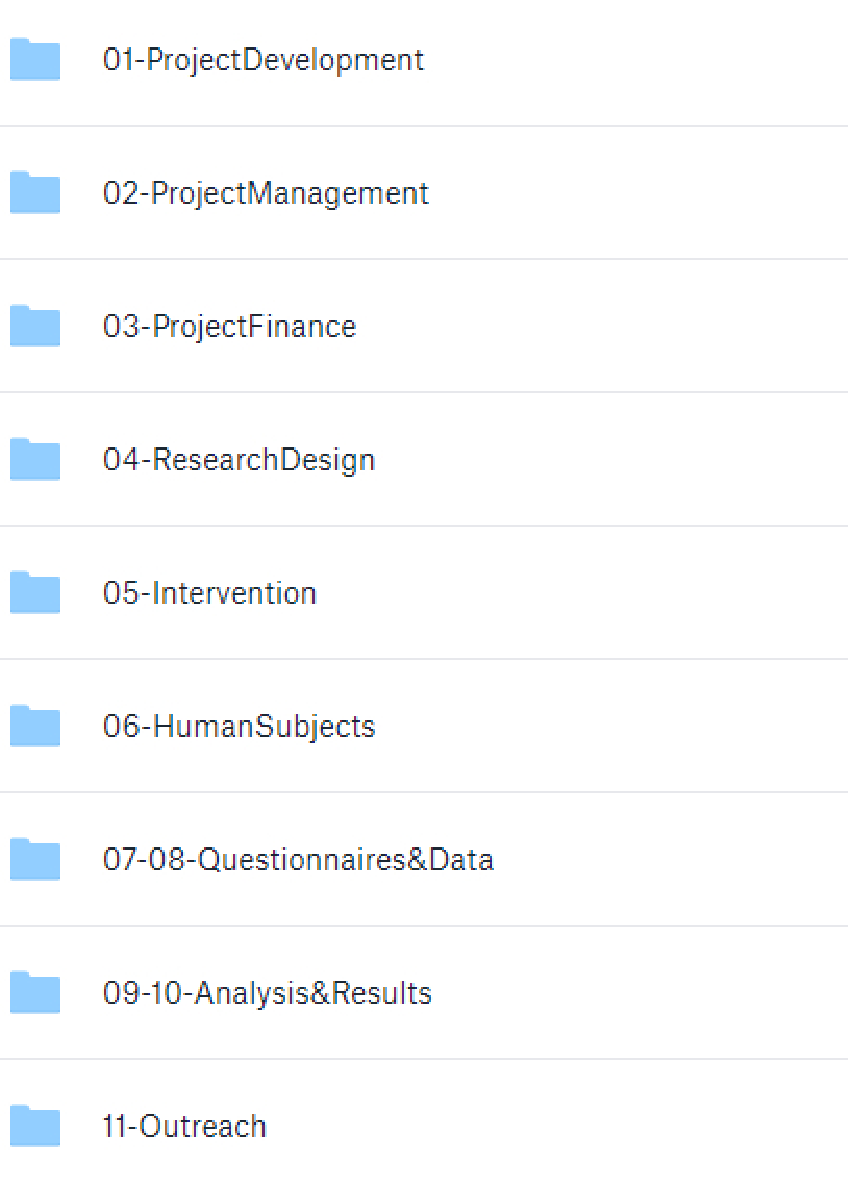
\includegraphics[width=0.35\textwidth]{fig1.pdf}
\end{figure}


\begin{figure}[htbp]
	\centering
	\caption{Estructura de las carpetas de datos y códigos. \label{fig:code}}
	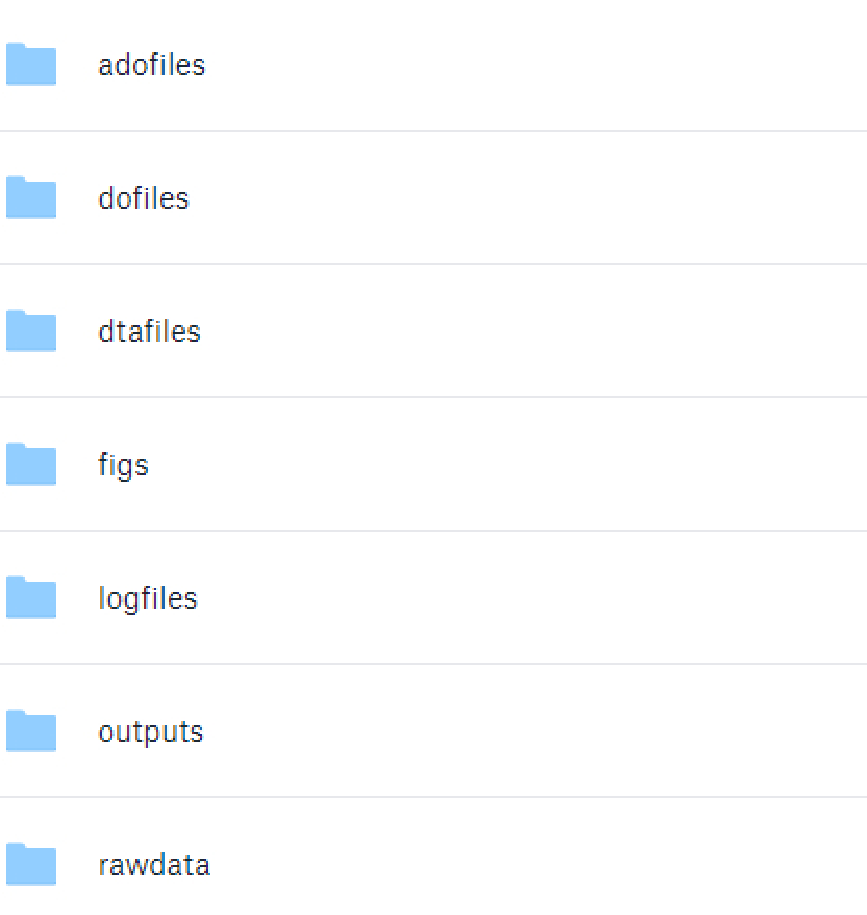
\includegraphics[width=0.35\textwidth]{fig2.pdf}
\end{figure}

%----------------------------------------------------------------------------------------
\end{document}
%----------------------------------------------------------------------------------------
